\ifdefined\COMPLETE
\else
\documentclass[12pt]{article}
\usepackage{tikz}
\usetikzlibrary{shapes, calc, arrows, through, intersections, decorations.pathreplacing, patterns}



\begin{document}
\fi

\def\alph{$2+\sqrt{5}$}
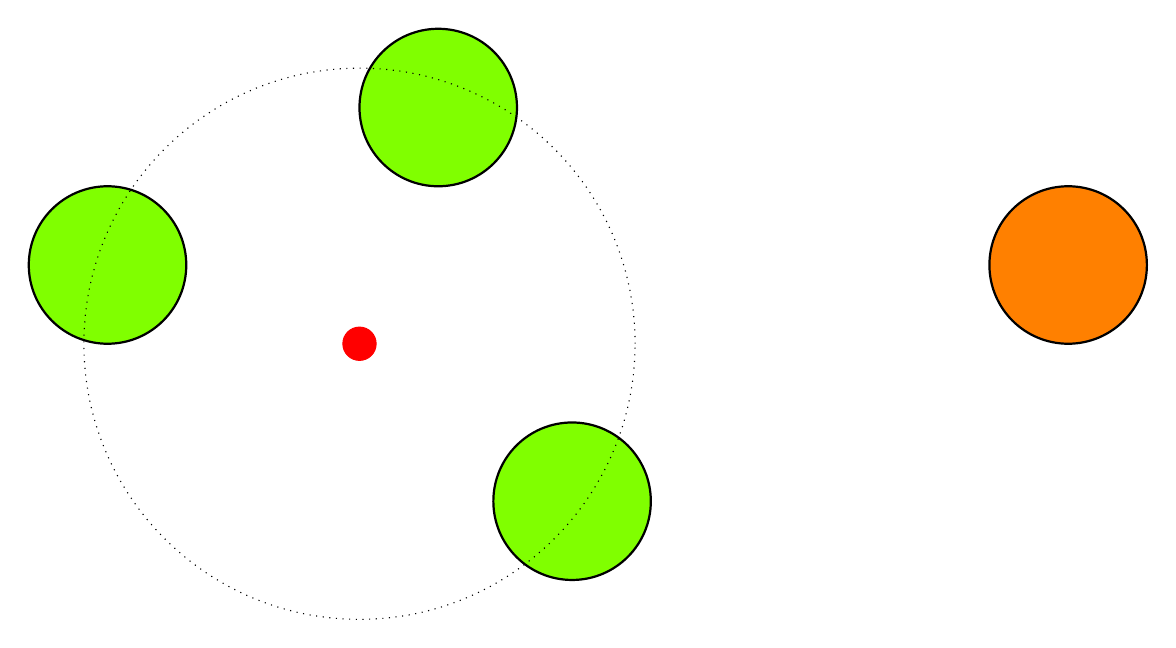
\begin{tikzpicture}
\draw[thick, fill={rgb:red,0;green,1;yellow,1}] (0.8,0) circle (1.0);
\draw[thick, fill={rgb:red,0;green,1;yellow,1}] (5.0,2.0) circle (1.0);
\draw[thick, fill={rgb:red,0;green,1;yellow,1}] (6.7,-3.0) circle (1.0);
\draw[thick, fill={rgb:red,1;green,0;yellow,1}] (13.0,0) circle (1.0);

\draw[black, dotted] (4.0,-1.0) circle (3.5);
\filldraw[red] (4.0,-1.0) circle (6pt) node[anchor=west] {};
\end{tikzpicture}

\ifdefined\COMPLETE
\else
\end{document}
\fi
